\documentclass{beamer}
\usetheme{Boadilla}

\usepackage{tikz}
\tikzset{
  font={\fontsize{8pt}{10}\selectfont}}
\usetikzlibrary{calc}
\usepackage{pgfplots}
\usetikzlibrary{pgfplots.groupplots}
\usetikzlibrary{matrix}

\definecolor{clstackoverflow}{HTML}{FE7A15}  
\definecolor{clgithub}{HTML}{4078C0} 

\graphicspath{ {../img/} }

\title{Convolutional neural networks
for classification of transmission
electron microscopy imagery}

\subtitle{}

\author{Sergii Gryshkevych}
\institute{Uppsala University}
\date{December 14, 2016}

\begin{document}

\begin{frame}
\titlepage
\end{frame}

\section{Introduction}

\begin{frame}
\frametitle{Introduction}
Introduction
\end{frame}

%
%	Performance measures
%

\begin{frame}
\frametitle{Performance measures}

\begin{block}{The Accuracy Paradox}
Models with a given accuracy may have greater predictive power than models with higher accuracy.
\end{block}

\begin{block}{Confusion matrix}
\begin{table}
\begin{tabular}{|c|c|c|}
\hline 
 & Predicted True & Predicted False \\ 
\hline 
Actual True & True Positive & False Negative \\ 
\hline 
Actual False & False Positive & True Negative \\ 
\hline 
\end{tabular} 
\end{table}
\end{block}


\end{frame}

\begin{frame}
\frametitle{Performance measures}

\begin{block}<1->{True positive rate (TPR)}
AKA sensitivity or recall: $TPR = \frac{TP}{TP + FN}$
\end{block}

\begin{block}<2->{True negative rate (TNR)}
AKA specificity: $TNR = \frac{TN}{TN + FP}$
\end{block}

\begin{block}<3->{Positive predicted value (PPV)}
AKA precision: $PPV = \frac{TP}{TP + FP}$
\end{block}

\begin{block}<4->{Negative predicted value (NPV)}
$NPV = \frac{TN}{TN + FN}$
\end{block}

\begin{block}<5->{$F_1$ score}
It is a harmonic mean of TPR and TNR
\end{block}

\end{frame}

%
%	Data augmentation
%

\section{Data augmentation}
\begin{frame}
\frametitle{Data augmentation techniques}

\begin{itemize}
\item<1-> Rotation in the range $[-180, 180]$ degrees with spline interpolation
\item<2-> Shear transformation in the range $[0, 0.2]$
\item<3-> Vertical shift in the range $[-10, 10]$ percent of total height
\item<4-> Horizontal shift in the range $[-10, 10]$ percent of total width
\item<5-> Zoom in the range $[0.8, 1.0]$ which means zoom by a maximum $20\%$
\item<6-> Horizontal flip
\item<7-> Vertical flip
\end{itemize}

\end{frame}

\begin{frame}
\frametitle{Data augmentation example}
\begin{figure}
\centering
\begin{tabular}{ccccc}
\includegraphics[scale=0.5]{augmented/541253.jpg} & \includegraphics[scale=0.5]{augmented/_0_645.jpeg} & \includegraphics[scale=0.5]{augmented/_0_1385.jpeg} & \includegraphics[scale=0.5]{augmented/_0_1749.jpeg} & \includegraphics[scale=0.5]{augmented/_0_2343.jpeg} \\

\includegraphics[scale=0.5]{augmented/_0_4050.jpeg} & \includegraphics[scale=0.5]{augmented/_0_3413.jpeg} & \includegraphics[scale=0.5]{augmented/_0_3414.jpeg} & \includegraphics[scale=0.5]{augmented/_0_3687.jpeg} & \includegraphics[scale=0.5]{augmented/_0_3916.jpeg} \\
	
\includegraphics[scale=0.5]{augmented/_0_4165.jpeg} & \includegraphics[scale=0.5]{augmented/_0_5014.jpeg} & \includegraphics[scale=0.5]{augmented/_0_5165.jpeg} & \includegraphics[scale=0.5]{augmented/_0_5567.jpeg} & \includegraphics[scale=0.5]{augmented/_0_6089.jpeg} \\

\includegraphics[scale=0.5]{augmented/_0_7140.jpeg} & \includegraphics[scale=0.5]{augmented/_0_7746.jpeg} & \includegraphics[scale=0.5]{augmented/_0_8553.jpeg} & \includegraphics[scale=0.5]{augmented/_0_8763.jpeg} & \includegraphics[scale=0.5]{augmented/_0_9361.jpeg} 
	
\end{tabular}
\end{figure}
\end{frame}

%
%	Effect of data augmentation
%

\begin{frame}
\frametitle{Effect of the data augmentation}

\begin{figure}
\centering

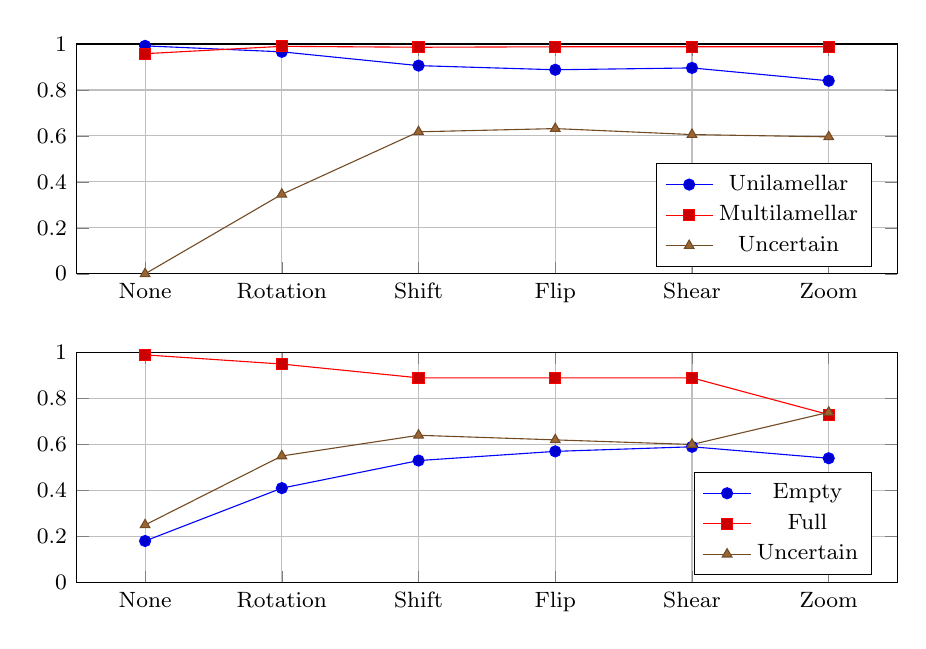
\begin{tikzpicture}
\begin{groupplot}[
	group style = {group size = 1 by 2, vertical sep=1cm,},
	width = 12cm,
	height = 4.5cm,
	grid=major,
    ymin=0.0,
    ymax=1.0,
    %ylabel=Average normalized true positive rate, 
    legend pos=south east,
    symbolic x coords={None, Rotation, Shift, Flip, Shear, Zoom},
    xtick=data,
    ]

% lamellarity
\nextgroupplot
\addplot+ [mark=*] coordinates{(None, 0.992) (Rotation, 0.966) (Shift, 0.906) (Flip, 0.888) (Shear, 0.896) (Zoom, 0.84)};
\addplot+ [mark=square*] coordinates{(None, 0.958) (Rotation, 0.99) (Shift, 0.986) (Flip, 0.988) (Shear, 0.988) (Zoom, 0.988)};
\addplot+ [mark=triangle*] coordinates{(None, 0.0) (Rotation, 0.346) (Shift, 0.618) (Flip, 0.632) (Shear, 0.606) (Zoom, 0.596)};

\legend{Unilamellar, Multilamellar, Uncertain}

% encapsulation
\nextgroupplot
\addplot+ [mark=*] coordinates{(None, 0.18) (Rotation, 0.41) (Shift, 0.53) (Flip, 0.57) (Shear, 0.59) (Zoom, 0.54)};
\addplot+ [mark=square*] coordinates{(None, 0.99) (Rotation, 0.95) (Shift, 0.89) (Flip, 0.89) (Shear, 0.89) (Zoom, 0.73)};
\addplot+ [mark=triangle*] coordinates{(None, 0.25) (Rotation, 0.55) (Shift, 0.64) (Flip, 0.62) (Shear, 0.6) (Zoom, 0.74)};
\legend{Empty, Full, Uncertain}

\end{groupplot}
\end{tikzpicture}
\end{figure}

\end{frame}

%
%	LipNet networks
%

\begin{frame}
\frametitle{Network architectures}

\begin{figure}
\centering
\includegraphics[width=\linewidth,height=0.8\textheight,keepaspectratio]{lipnet_architecture.png} 
\end{figure}

\end{frame}


%
%	Popularity of DL software
%

\begin{frame}
\frametitle{Popularity of deep learning software as of October 2016}
\begin{figure}[H]
\centering

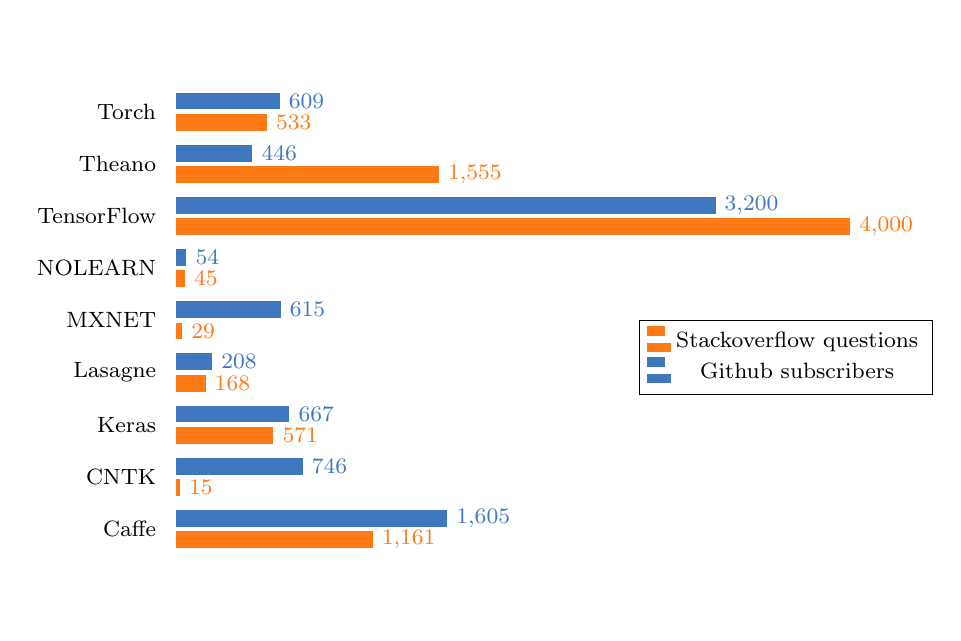
\begin{tikzpicture}
\begin{axis}[
	xbar,
	y axis line style = { opacity = 0 },
	axis x line = none,
	tickwidth = 0pt,
	enlarge y limits = 0.2,
	enlarge x limits = 0.02,
	bar width = 0.2cm,
	symbolic y coords = {Caffe, CNTK, Keras, Lasagne, MXNET, NOLEARN, TensorFlow, Theano, Torch},
	ytick = data,
	nodes near coords,
	height = 9cm,
	legend style={at={(1.1, 0.5)},anchor=north east}
    ]

% stackoverflow
\addplot[color=clstackoverflow, fill=clstackoverflow] coordinates{(1161,Caffe) (15,CNTK) (571,Keras) (168,Lasagne) (29,MXNET) (45,NOLEARN) (4000,TensorFlow) (1555,Theano) (533,Torch)};

% github
\addplot[color=clgithub, fill=clgithub] coordinates{(1605,Caffe) (746,CNTK) (667,Keras) (208,Lasagne) (615,MXNET) (54,NOLEARN) (3200,TensorFlow) (446,Theano) (609,Torch)};

\legend{Stackoverflow questions, Github  subscribers}

\end{axis}
\end{tikzpicture}

\end{figure}
\end{frame}

%
%	CNN vs SVM
%

\section{Benchmarking}

\begin{frame}
\frametitle{CNN vs SVM: Lamellarity}

\begin{figure}
\centering
\includegraphics[width=\linewidth,height=0.8\textheight,keepaspectratio]{cnn_vs_svm_lamellarity.png} 
\end{figure}

\end{frame}

\begin{frame}
\frametitle{CNN vs SVM: Encapsulation}

\begin{figure}
\centering
\includegraphics[width=\linewidth,height=0.8\textheight,keepaspectratio]{cnn_vs_svm_encapsulation.png} 
\end{figure}

\end{frame}

\end{document}